%! Author = Main
%! Date = 05.02.2020

% Preamble
\documentclass{beamer}
\usetheme{Darmstadt}

% Packages
\usepackage{ngerman}
\usepackage{color} % Colored font
\usepackage{graphicx} % Images
\usepackage{titling} % Title formatting
\usepackage[utf8]{inputenc} % UTF-8
\usepackage {tikz}
\usepackage{amsmath} % Graphs
\usepackage{etoolbox} % Well formatted Links in bib
\apptocmd{\thebibliography}{\raggedright}{}{} % Well formatted Links in bib
\usepackage{hyperref} % Links

% Meta information
\title{\Huge{Intelligente Systeme}}
\subtitle{\Large - Referat -}
\author{Adrian Helberg}
\institute{HAW Hamburg}
\date{21.02.2020}
\titlegraphic{
\begin{picture}
    (0,0)
    % -56,20: Bottom left
    \put(-56,212){\makebox(0,0)[rt]{
\includegraphics[width=3.8cm]{../../resources/Haw_logo.png}}}
    \put(158,200){\makebox(0,0)[rt]{
\includegraphics[width=5cm]{../../resources/fakultaet.PNG}}}
\end{picture}
}

\newenvironment<>{definition}[1]{%
    \setbeamercolor{block title}{fg=white,bg=green!75!black}%
    \begin{block}#2{#1}}{\end{block}}

% Slides
\begin{document}
    \frame{\titlepage}

    \frame{
    \frametitle{Inhalt}
    \tableofcontents
    }

    \section{Suchen}
    \frame{
    \frametitle{Problem des Handlungsreisenden}
        \begin{definition}{Definition}
            Die Aufgabe besteht darin, eine Reihenfolge für den Besuch mehrerer Orte so zu wählen,
            dass keine Station außer der ersten mehr als einmal besucht wird, die gesamte
            Reisestrecke des Handlungsreisenden möglichst kurz und die erste Station gleich der
            letzten Station ist \footnotemark
        \end{definition}
        \footnotetext[1]{\url{https://de.wikipedia.org/wiki/Problem_des_Handlungsreisenden}}

        \begin{itemize}
            \setlength\itemsep{0.6em}
            \item Kombinatorisches Optimierungsproblem
            \item $10!=3628800$ mögliche Lösungen
            \item Theoretische Informatik
            \item Festlegung der Reihenfolge der zu besuchenden Städte
            \item NP-vollständig
        \end{itemize}
    }

    \frame{
        \frametitle{Genetischer Algorithmus}
        \begin{definition}{Definition}
            Evolutionäre Algorithmen (EA) sind eine Klasse von stochastischen, metaheuristischen
            Optimierungsverfahren, deren Funktionsweise von der Evolution natürlicher Lebewesen
            inspiriert ist \footnotemark
        \end{definition}
        \footnotetext[2]{\url{https://de.wikipedia.org/wiki/Evolutionarer_Algorithmus}}

        \begin{itemize}
            \setlength\itemsep{1em}
            \item Optimierte, akzeptable Lösung
            \item Aufgabenstellung mit hoher kombinatorischen Komplexität
            \item Mengen an (immer besser werdenden) Lösungen
            \item Kein "`Hängenbleiben"' an einem lokalen Optimum
        \end{itemize}
    }

    \frame{
        \frametitle{Ablauf (1/2)}
        \begin{center}
            \begin{tikzpicture}[semithick , state/.style ={ rectangle ,top color =white , bottom color = processblue!20 ,
            draw,processblue , text=blue , minimum width =1 cm}]
                \node[state] (A) at (0,0) {Start};
                \node[state] (B) at (0,-1.2) {Erzeugung einer zufälliger Population};
                \node[state] (C) at (0,-2.4) {Wiederhole bis Abbruchbedungung erfüllt};
                \node[state] (D) at (0,-3.6) {Berechne Fitness};
                \node[state] (E) at (0,-4.8) {Selektion};

                \draw[->, very thick] (A) to (B);
                \draw[->, very thick] (B) to (C);
                \draw[->, very thick] (C) to (D);
                \draw[->, very thick] (D) to (E);
            \end{tikzpicture}
        \end{center}
    }

    \frame{
        \frametitle{Ablauf (2/2)}
        \begin{center}
            \begin{tikzpicture}[semithick , state/.style ={ rectangle ,top color =white , bottom color = processblue!20 ,
            draw,processblue , text=blue , minimum width =1 cm}]
                \node[state] (F) at (0,0) {Crossover};
                \node[state] (G) at (0,-1.2) {Mutation};
                \node[state] (H) at (0,-2.4) {Austausch};
                \node[state] (I) at (0,-3.6) {Teste Abbruchbedingung};
                \node[state] (J) at (0,-4.8) {Ende};

                \draw[->, very thick] (F) to (G);
                \draw[->, very thick] (G) to (H);
                \draw[->, very thick] (H) to (I);
                \draw[->, very thick] (I) to (J);
            \end{tikzpicture}
        \end{center}
    }

    \frame{
        \frametitle{Eigenschaften}
        \begin{itemize}
            \setlength\itemsep{1.6em}
            \item Chromosomen
            \item Fitness
            \item Selektion
            \item Kreuzung
            \item Mutation
            \item Austausch
        \end{itemize}
    }

    \frame{
        \frametitle{Realisierung mit Java}
        \begin{center}
            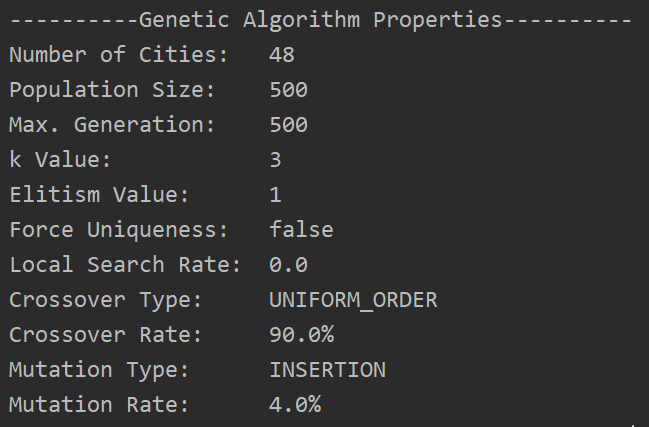
\includegraphics[width=10cm]{../../resources/properties_algorithm.png}
        \end{center}
    }

    \section{Lernen}
    \frame{
        \frametitle{Selbstorganierende Karte}
        \begin{definition}{Definition}
            Als Selbstorganisierende Karten $[...]$ bezeichnet man eine Art von künstlichen
            neuronalen Netzen. $[...]$ Ihr Funktionsprinzip beruht auf der biologischen Erkenntnis,
            dass viele Strukturen im Gehirn eine lineare oder planare Topologie aufweisen
            \footnotemark
        \end{definition}
        \footnotetext[3]{\url{https://de.wikipedia.org/wiki/Selbstorganisierende_Karte}}

        \begin{itemize}
            \setlength\itemsep{0.6em}
            \item Neuroinformatik
            \item \textit{Kohonen}-Karte, \textit{SOM}
            \item Unüberwachtes Lernen
        \end{itemize}
    }

    \section{Sequenzen}
    \frame{
    \frametitle{Sequenzen}
    A Deep Learning Approach to on-Node Sensor
    Data Analytics for Mobile or Wearable Devices
    }

    \section{Quellen}
    \frame{
    \frametitle{Quellen}
        \bibliographystyle{plain}
        \bibliography{script}
    }

\end{document}